% Options for packages loaded elsewhere
% Options for packages loaded elsewhere
\PassOptionsToPackage{unicode}{hyperref}
\PassOptionsToPackage{hyphens}{url}
\PassOptionsToPackage{dvipsnames,svgnames,x11names}{xcolor}
%
\documentclass[
]{article}
\usepackage{xcolor}
\usepackage{amsmath,amssymb}
\setcounter{secnumdepth}{-\maxdimen} % remove section numbering
\usepackage{iftex}
\ifPDFTeX
  \usepackage[T1]{fontenc}
  \usepackage[utf8]{inputenc}
  \usepackage{textcomp} % provide euro and other symbols
\else % if luatex or xetex
  \usepackage{unicode-math} % this also loads fontspec
  \defaultfontfeatures{Scale=MatchLowercase}
  \defaultfontfeatures[\rmfamily]{Ligatures=TeX,Scale=1}
\fi
\usepackage{lmodern}
\ifPDFTeX\else
  % xetex/luatex font selection
\fi
% Use upquote if available, for straight quotes in verbatim environments
\IfFileExists{upquote.sty}{\usepackage{upquote}}{}
\IfFileExists{microtype.sty}{% use microtype if available
  \usepackage[]{microtype}
  \UseMicrotypeSet[protrusion]{basicmath} % disable protrusion for tt fonts
}{}
\makeatletter
\@ifundefined{KOMAClassName}{% if non-KOMA class
  \IfFileExists{parskip.sty}{%
    \usepackage{parskip}
  }{% else
    \setlength{\parindent}{0pt}
    \setlength{\parskip}{6pt plus 2pt minus 1pt}}
}{% if KOMA class
  \KOMAoptions{parskip=half}}
\makeatother
% Make \paragraph and \subparagraph free-standing
\makeatletter
\ifx\paragraph\undefined\else
  \let\oldparagraph\paragraph
  \renewcommand{\paragraph}{
    \@ifstar
      \xxxParagraphStar
      \xxxParagraphNoStar
  }
  \newcommand{\xxxParagraphStar}[1]{\oldparagraph*{#1}\mbox{}}
  \newcommand{\xxxParagraphNoStar}[1]{\oldparagraph{#1}\mbox{}}
\fi
\ifx\subparagraph\undefined\else
  \let\oldsubparagraph\subparagraph
  \renewcommand{\subparagraph}{
    \@ifstar
      \xxxSubParagraphStar
      \xxxSubParagraphNoStar
  }
  \newcommand{\xxxSubParagraphStar}[1]{\oldsubparagraph*{#1}\mbox{}}
  \newcommand{\xxxSubParagraphNoStar}[1]{\oldsubparagraph{#1}\mbox{}}
\fi
\makeatother


\usepackage{longtable,booktabs,array}
\usepackage{calc} % for calculating minipage widths
% Correct order of tables after \paragraph or \subparagraph
\usepackage{etoolbox}
\makeatletter
\patchcmd\longtable{\par}{\if@noskipsec\mbox{}\fi\par}{}{}
\makeatother
% Allow footnotes in longtable head/foot
\IfFileExists{footnotehyper.sty}{\usepackage{footnotehyper}}{\usepackage{footnote}}
\makesavenoteenv{longtable}
\usepackage{graphicx}
\makeatletter
\newsavebox\pandoc@box
\newcommand*\pandocbounded[1]{% scales image to fit in text height/width
  \sbox\pandoc@box{#1}%
  \Gscale@div\@tempa{\textheight}{\dimexpr\ht\pandoc@box+\dp\pandoc@box\relax}%
  \Gscale@div\@tempb{\linewidth}{\wd\pandoc@box}%
  \ifdim\@tempb\p@<\@tempa\p@\let\@tempa\@tempb\fi% select the smaller of both
  \ifdim\@tempa\p@<\p@\scalebox{\@tempa}{\usebox\pandoc@box}%
  \else\usebox{\pandoc@box}%
  \fi%
}
% Set default figure placement to htbp
\def\fps@figure{htbp}
\makeatother





\setlength{\emergencystretch}{3em} % prevent overfull lines

\providecommand{\tightlist}{%
  \setlength{\itemsep}{0pt}\setlength{\parskip}{0pt}}



 


\makeatletter
\@ifpackageloaded{caption}{}{\usepackage{caption}}
\AtBeginDocument{%
\ifdefined\contentsname
  \renewcommand*\contentsname{Table of contents}
\else
  \newcommand\contentsname{Table of contents}
\fi
\ifdefined\listfigurename
  \renewcommand*\listfigurename{List of Figures}
\else
  \newcommand\listfigurename{List of Figures}
\fi
\ifdefined\listtablename
  \renewcommand*\listtablename{List of Tables}
\else
  \newcommand\listtablename{List of Tables}
\fi
\ifdefined\figurename
  \renewcommand*\figurename{Figure}
\else
  \newcommand\figurename{Figure}
\fi
\ifdefined\tablename
  \renewcommand*\tablename{Table}
\else
  \newcommand\tablename{Table}
\fi
}
\@ifpackageloaded{float}{}{\usepackage{float}}
\floatstyle{ruled}
\@ifundefined{c@chapter}{\newfloat{codelisting}{h}{lop}}{\newfloat{codelisting}{h}{lop}[chapter]}
\floatname{codelisting}{Listing}
\newcommand*\listoflistings{\listof{codelisting}{List of Listings}}
\makeatother
\makeatletter
\makeatother
\makeatletter
\@ifpackageloaded{caption}{}{\usepackage{caption}}
\@ifpackageloaded{subcaption}{}{\usepackage{subcaption}}
\makeatother
\usepackage{bookmark}
\IfFileExists{xurl.sty}{\usepackage{xurl}}{} % add URL line breaks if available
\urlstyle{same}
\hypersetup{
  pdftitle={Database-Agnostic Machine Learning},
  pdfauthor={Vinay Valson},
  colorlinks=true,
  linkcolor={blue},
  filecolor={Maroon},
  citecolor={Blue},
  urlcolor={Blue},
  pdfcreator={LaTeX via pandoc}}


\title{Database-Agnostic Machine Learning}
\author{Vinay Valson}
\date{2026-01-20}
\begin{document}
\maketitle

\renewcommand*\contentsname{Table of contents}
{
\hypersetup{linkcolor=}
\setcounter{tocdepth}{3}
\tableofcontents
}

Do you have a database? Do you want to make predictions without the
hassles of having data scientists? I got you covered!

\subsection{The Challenge with Relational
Data}\label{the-challenge-with-relational-data}

Most companies store their data in relational databases. These are
systems that organize information into tables, like spreadsheets, which
can be linked together using keys - like connecting a ``Customers''
table with an ``Orders'' table. While this structure is great for
storing large amounts of data efficiently, it can be challenging when
you want to use machine learning to make predictions or gain insights.

Traditionally, machine learning models expect all the data in a single,
flat table. This means analysts have to manually combine tables,
calculate summary statistics, and create new ``features'' from the raw
data. This is a process that is very time consuming, error-prone, and
specific to each database. If a database changes even slightly, the
model may break, and all the work has to be redone - fyi job of the data
scientist.

\begin{figure}[H]

{\centering \pandocbounded{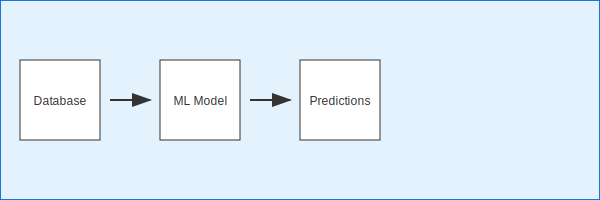
\includegraphics[keepaspectratio]{placeholder-pipeline.png}}

}

\caption{Data Science Pipeline}

\end{figure}%

\subsection{The Solution: Database-Agnostic Machine
Learning}\label{the-solution-database-agnostic-machine-learning}

The solution is database-agnostic machine learning, which allows models
to work directly with relational data without manual preparation.
``Agnostic'' here means flexible and the model can work across different
database structures without needing to be customized for each one.

\begin{figure}[H]

{\centering \pandocbounded{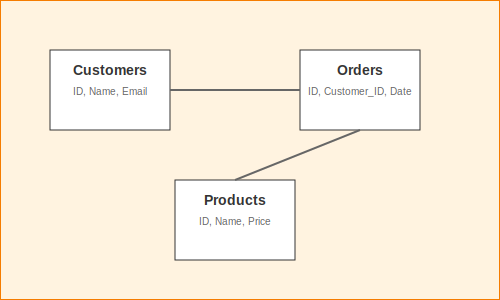
\includegraphics[keepaspectratio]{placeholder-schema.png}}

}

\caption{Relational Database Schema}

\end{figure}%

\subsection{Graph Transformers: Beyond
Databases}\label{graph-transformers-beyond-databases}

Graph transformers are a powerful architecture that extends the
transformer model (famous from GPT and BERT) to work with
graph-structured data. While traditional transformers work on sequences
(like sentences), graph transformers can process nodes and edges in a
graph.

\textbf{Where else are graph transformers used?}

\begin{itemize}
\tightlist
\item
  \textbf{Social Networks:} Predicting user behavior and connections on
  platforms like Facebook or LinkedIn, where users are nodes and
  friendships are edges
\item
  \textbf{Drug Discovery:} Modeling molecular structures where atoms are
  nodes and chemical bonds are edges, helping researchers predict drug
  properties
\item
  \textbf{Traffic Prediction:} Understanding road networks where
  intersections are nodes and roads are edges, enabling better route
  planning
\item
  \textbf{Recommendation Systems:} Connecting users, products, and
  interactions in e-commerce platforms to suggest relevant items
\item
  \textbf{Knowledge Graphs:} Organizing and reasoning over facts and
  relationships, like Google's Knowledge Graph
\end{itemize}

\begin{figure}[H]

{\centering \pandocbounded{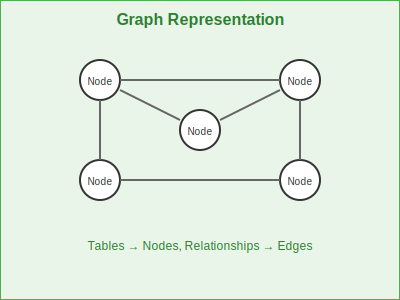
\includegraphics[keepaspectratio]{placeholder-graph.gif}}

}

\caption{Graph Transformer Visulization}

\end{figure}%

\subsection{KumoRFM: A Real-World
Example}\label{kumorfm-a-real-world-example}

A real-world example of this approach is \textbf{KumoRFM}, a tool that
works like a ``foundation model'' for relational data. Think of it as a
large language model but for structured business data instead of text.
KumoRFM represents tables and their relationships as a graph, where each
row is a point (node) and connections between tables are lines (edges).
Using a graph transformer, the model can automatically learn patterns
and relationships across tables, so it understands the structure and
meaning of the data.

\begin{figure}[H]

{\centering \pandocbounded{\includegraphics[keepaspectratio]{placeholder-kumo.png}}

}

\caption{Key capabilities of RFM}

\end{figure}%

\subsection{Key Advantages}\label{key-advantages}

This approach has several advantages:

\begin{itemize}
\tightlist
\item
  \textbf{No Complex Queries:} Analysts no longer need to write complex
  SQL queries or manually engineer features
\item
  \textbf{Instant Predictions:} Models can generate predictions
  instantly for new questions
\item
  \textbf{Universal Application:} The same approach can be applied
  across different databases and organizations
\item
  \textbf{Reduced Errors:} Eliminates manual data preparation mistakes
\item
  \textbf{Time Savings:} Allows analysts to focus on interpreting
  results rather than preparing data
\end{itemize}

\begin{figure}[H]

{\centering \pandocbounded{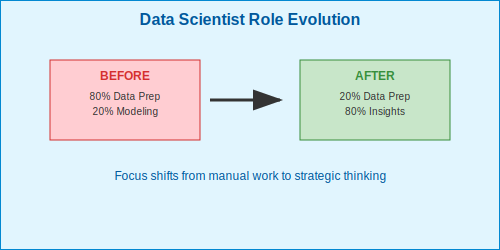
\includegraphics[keepaspectratio]{index_files/mediabag/placeholder-transformation.pdf}}

}

\caption{Role Transformation}

\end{figure}%

\subsection{The Impact}\label{the-impact}

In short, database-agnostic machine learning allows businesses to unlock
the full value of their relational data in a way that is fast, reliable,
and scalable. Tools like KumoRFM demonstrate that it's possible to
combine advanced machine learning with the complex structure of
relational databases, making insights more accessible and actionable for
decision makers.

As a result, this shift transforms the role of data scientists from
manual feature engineering to higher-level problem formulation and
decision-making.

\subsection{References}\label{references}

\begin{itemize}
\tightlist
\item
  \href{https://www.youtube.com/watch?v=xzv0-wgQVSA}{KumoRFM Video
  Introduction}
\item
  \href{https://kumorfm.ai/get-started}{KumoRFM Getting Started}
\item
  \href{https://medium.com/@kumo.ai/from-megawatt-errors-to-millions-saved-slashing-utility-costs-with-kumo-rfm-94a790294a33}{Case
  Study: Slashing Utility Costs with KumoRFM}
\end{itemize}




\end{document}
